\section{Background and Challenges}
\label{sec:challenges}

In this section, we discuss closely related work and how it fails to
address several open challenges for \emph{root cause}
analysis, \ie identifying the AS that originates a routing change
in the Internet.\footnotemark{} We discuss other related work in \S\ref{sec:related}.

\footnotetext{We do \emph{not} identify reasons for a routing
change, \eg whether a change was caused by a link failure or traffic
engineering.}

\subsection{\feldmannbold Approach}

The first general approach for root cause analysis was proposed by Feldmann et al.~\cite{feldman}.  The
key idea behind this heuristic is that the root cause of a path change
observed at an AS is likely either on the old path used before the change or
the new path used after the change. We refer to this approach as
\feldmann, because it identifies changes on the New Or Old Route. (We
use the terms `route' and `path' interchangeably in this paper.) The heuristic 
then combines simultaneous path change observations from
different ASes and builds a suspect set containing the ASes that appear
in all paths that changed and that never appear in paths that did not
change. Although not evaluated explicitly, to reduce the set of suspect
ASes further, \feldmann assumes that the root cause is on the most
preferred path (otherwise AS $A$ would keep using the preferred path and
there would be no change). 


The authors use simulation to inform their design, then evaluate their approach using 
experiments on real-world data with BGP beacons announcements for ground truth. 
In this context, Feldmann et al.~were able to isolate the origin of a
BGP path change to a single AS or inter-AS link for 76\% of the cases
they study. Applying further heuristics, they achieve this precision 
in 96\% of cases.
While these results may suggest that we can close the book
on root cause analysis, we list several challenges below that may impact
\feldmann's accuracy and precision.


\subsection{Open Challenges}

\begin{figure}[t]
\centering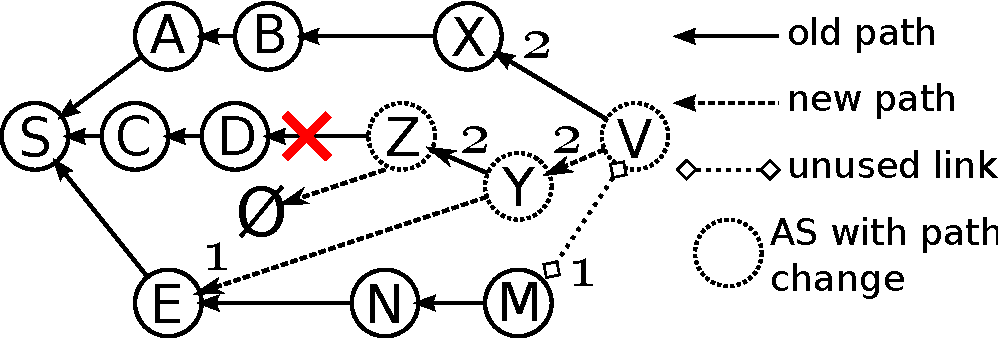
\includegraphics[width=\columnwidth]{figs/induced2.pdf}
\vspace{-2em}
\caption{Example of an induced path change at $\boldsymbol{v}$ after the
link $\boldsymbol{d}$--$\boldsymbol{z}$ fails.  Numbers on edges show
the local preference (LocalPref) of a peer, higher is more preferred.}
\label{fig:induced1}
\end{figure}

\nparagraph{Induced Path Changes.}  The root cause of a path
change observed at an AS $v$ may lie outside the old and new paths used
by $v$.  Feldmann et al.~\cite{feldman} recognize this challenge but did not have 
an approach to address it.  \fig~\ref{fig:induced1} shows an example network topology where
an induced change happens.  The solid arrows show the paths ASes chose
toward $s$ before the link between ASes $d$ and $z$ failed.  The dashed
arrows show the path ASes chose to AS $s$ after the failure.  ASes with
one outgoing arrow (solid circles) did not change paths.
Note that, before the failure, AS $y$ prefers the longer route
through $z$ (LocalPref~2, higher is more preferred) than the shorter route through $e$
(LocalPref~1).  When the failure happens, AS~$z$ cannot find a path to~$s$
and withdraws its path.  AS~$y$ then changes to the shorter, less
preferred route through $e$.  When $y$ announces the new route to $v$,
AS~$v$ changes to the new route $[y, e, s]$ because it is shorter than
the route through~$x$.  Note that the root cause, \ie the link between
ASes~$d$ and~$z$, does not lie in either the old or the new path used by
AS~$v$.  \feldmann cannot identify the root cause of induced path
changes; at best, it would find the AS where the change was induced,
\eg AS $y$.  Moreover, because \feldmann correlates changes across all
observation points, it suffices that one observation point experiences
an induced path change to make identification fail. We address such 
cascading path changes in \S\ref{subsec:rules}.


\nparagraph{Extensive Path Monitoring.}  BGP limits the amount of path-change 
information one can gather passively~\cite{routeviews, bgpmon}. For example, 
an AS that receives updated paths from different
downstream neighbors will forward only its best path upstream. One
consequence is that BGP and traceroute measurements from a small number of 
vantage points are insufficient to observe an arbitrary path change. 
We potentially need BGP measurements from each AS
in the network~\cite{teixeira04omni}, or techniques such as Reverse Traceroute~\cite{revtr} that provide path
measurements from arbitrary ASes, to have complete
information to perform root cause analysis.  We determine the set of
required measurements in 
\S\ref{subsec:canopy} then use a simple routing model to bound this set
in \S\ref{subsec:bound}.

\nparagraph{Inferring Route Preferences.}  When an AS switches from path
$P$ to $P^\prime$, it may be unclear which of the two paths it prefers.
Feldmann et al.~proposed a heuristic that considers the
shorter path the preferred path. However, in practice inter-AS business
relationships (\ie policy routing) take precedence over path length in
the route selection process. Incorrect assumptions about routing policies 
can prevent root cause analysis from identifying the correct AS responsible for 
a path change. We describe our preference inference mechanism in
\S\ref{subsec:bound}.


\begin{comment}
\nparagraph{Measurement Granularity.}  Most previous work focuses
on isolating the root cause of path changes to an AS; however, this
coarse grained analysis can be insufficient for two reasons. First,
different routers in the same AS may use different routes toward the
same prefix.  For example, a router in Europe is likely to choose
different routes than a router in the US, even if they belong to the
same AS.  Second, when debugging performance or connectivity problems,
fine-grained isolation of the root cause (\eg at the level of
point-of-presence or router IP) can speed diagnosis and repair by
focusing limited operator resources on a narrow region of the network. 
\drc{May need to cut this if we can't say that we actually address this.}
\end{comment}

%In the next section, we develop a model of path changes that accounts
%for root causes in arbitrary locations, addressing the first and second
%challenges.  In Section~\ref{sec:design} we design a system that
%addresses the remaining challenges using extensive data- and
%control-plane measurements. 
